\documentclass[9pt,a4paper]{extarticle}
\usepackage[a4paper,left=1.5cm,right=1.5cm,top=1.3cm,bottom=1.3cm]{geometry}
% Shared layout for report and factsheet (pdflatex, standard TeX Live / Overleaf packages)
\usepackage[T1]{fontenc}
\usepackage[utf8]{inputenc}
\usepackage[sc]{mathpazo}
\usepackage[scaled=0.9]{helvet}
\usepackage{microtype}
\usepackage{amsmath}
\usepackage{booktabs}
\usepackage{array}
\usepackage{tabularx}
\usepackage{graphicx}
\usepackage{xcolor}
\usepackage{enumitem}
\usepackage{caption}
\usepackage{titlesec}
\usepackage{fancyhdr}
\usepackage[hidelinks]{hyperref}

\definecolor{accent}{HTML}{1C5CAB}
\definecolor{muted}{HTML}{52514E}
\definecolor{rulegrey}{HTML}{C9C8C3}
\definecolor{panel}{HTML}{F3F2EE}

\newcommand{\TeamName}{Team Backwardation}
\newcommand{\TeamMembers}{Lukas Lobnig, Niklas Omann, Noemi Pirrello, Adrian Rupp}
\newcommand{\ProjectTitle}{Earning the Roll}
\newcommand{\ProjectSubtitle}{A volatility-targeted carry strategy for WTI crude oil futures}

% generated by wti.report - do not edit
\newcommand{\NNDaily}{9{,}145}
\newcommand{\NNWeekly}{1{,}909}
\newcommand{\NNRolls}{472}
\newcommand{\NRollAgree}{87\%}
\newcommand{\NRollAgreeN}{218}
\newcommand{\NRollBefore}{9\%}
\newcommand{\NRollAfter}{19\%}
\newcommand{\NKurtDaily}{16.5}
\newcommand{\NKurtMonthly}{2.4}
\newcommand{\NKurtResid}{2.2}
\newcommand{\NAcfAbsHundred}{0.06}
\newcommand{\NGarchSpec}{EGARCH-t}
\newcommand{\NGarchPersist}{0.991}
\newcommand{\NGarchNu}{6.8}
\newcommand{\NGarchGammaT}{\textminus 3.9}
\newcommand{\NGarchBicGain}{39}
\newcommand{\NDmEwmaP}{$<$0.001}
\newcommand{\NDmRollP}{$<$0.001}
\newcommand{\NDmNormalP}{0.316}
\newcommand{\NOvxCorr}{0.92}
\newcommand{\NVarLags}{4}
\newcommand{\NBicLags}{1}
\newcommand{\NAicLags}{8}
\newcommand{\NLbSlopeOne}{$<$0.001}
\newcommand{\NLbMinFour}{0.12}
\newcommand{\NGrangerAllP}{0.374}
\newcommand{\NGrangerSlopeP}{0.635}
\newcommand{\NPassSum}{0.0078}
\newcommand{\NPassZeroP}{0.482}
\newcommand{\NPassFullP}{0.305}
\newcommand{\NBackAnn}{26.7}
\newcommand{\NBackT}{3.1}
\newcommand{\NContAnn}{\textminus 14.1}
\newcommand{\NContT}{\textminus 1.2}
\newcommand{\NIrfSlopeInvImpact}{\textminus 0.72}
\newcommand{\NIrfSlopeInvTwelve}{\textminus 0.46}
\newcommand{\NIrfRetInvImpact}{\textminus 0.40}
\newcommand{\NIrfRetInvTwelve}{\textminus 0.29}
\newcommand{\NIrfRetSlopeImpact}{2.85}
\newcommand{\NIrfRetSlopeTwelve}{3.53}
\newcommand{\NIrfDrift}{0.68}
\newcommand{\NIrfDriftLo}{\textminus 0.25}
\newcommand{\NIrfDriftHi}{1.35}
\newcommand{\NSlopeSd}{6.1}
\newcommand{\NWeeklyVolIs}{4.6}
\newcommand{\NCarryWeekIs}{0.28}
\newcommand{\NBenchVolIs}{36.5\%}
\newcommand{\NOosRtwoVal}{\textminus 2.0\%}
\newcommand{\NOosRtwoOos}{\textminus 2.6\%}
\newcommand{\NCwPOos}{0.819}
\newcommand{\NVarShareLong}{58\%}
\newcommand{\NNTrials}{26}
\newcommand{\NDsrHurdle}{0.60}
\newcommand{\NDsr}{63\%}
\newcommand{\NTargetVol}{35\%}
\newcommand{\NMaxLev}{2}
\newcommand{\NFreezeCommit}{9fb1e8d}
\newcommand{\NHolmMain}{0.282}
\newcommand{\NPsrMainP}{0.056}
\newcommand{\NBootLo}{0.02}
\newcommand{\NBootHi}{0.86}
\newcommand{\NBootP}{0.040}
\newcommand{\NBootDiff}{0.38}
\newcommand{\NBootDiffLo}{\textminus 0.29}
\newcommand{\NBootDiffHi}{1.04}
\newcommand{\NBootDiffP}{0.177}
\newcommand{\NSubOne}{0.22}
\newcommand{\NSubTwo}{0.45}
\newcommand{\NSubThree}{0.58}
\newcommand{\NRobMin}{0.18}
\newcommand{\NRobMax}{0.52}
\newcommand{\NRobN}{15}
\newcommand{\NRobFiveTicks}{0.36}
\newcommand{\NRobLongFlat}{0.31}
\newcommand{\NRobLongFlatDd}{\textminus 43\%}
\newcommand{\NRobMonthly}{0.27}
\newcommand{\NRobBand}{0.18}
\newcommand{\NRobTwoThree}{0.52}
\newcommand{\NVarHitBench}{1.54\%}
\newcommand{\NVarKupBench}{0.003}
\newcommand{\NVarHitMain}{0.73\%}
\newcommand{\NVarKupMain}{0.089}
\newcommand{\NVarHitsBench}{55}
\newcommand{\NVarDaysBench}{3{,}574}
\newcommand{\NSkewOos}{\textminus 3.6}
\newcommand{\NStressCovid}{20\%}
\newcommand{\NStressCovidBench}{\textminus 78\%}
\newcommand{\NStressOpec}{45\%}
\newcommand{\NStressOpecBench}{\textminus 74\%}
\newcommand{\NStressRussia}{29\%}
\newcommand{\NValSharpeBench}{0.50}
\newcommand{\NValSharpeLongVol}{0.55}
\newcommand{\NValSharpeVar}{0.14}
\newcommand{\NValSharpeVarVol}{0.02}
\newcommand{\NValSharpeCarry}{0.74}
\newcommand{\NValSharpeMain}{0.70}
\newcommand{\NValCagrMain}{21.9\%}
\newcommand{\NValVolMain}{36\%}
\newcommand{\NValMddMain}{\textminus 54\%}
\newcommand{\NValMddBench}{\textminus 78\%}
\newcommand{\NValCagrBench}{14.7\%}
\newcommand{\NValAlphaMain}{23.7\%}
\newcommand{\NValAlphaT}{2.3}
\newcommand{\NValBetaMain}{0.08}
\newcommand{\NValTurnMain}{33}
\newcommand{\NValCostMain}{1.41\%}
\newcommand{\NValLongMain}{56\%}
\newcommand{\NValSharpeSe}{0.29}
\newcommand{\NValEsMain}{7.8\%}
\newcommand{\NValEsBench}{8.5\%}
\newcommand{\NOosSharpeBench}{0.03}
\newcommand{\NOosSharpeLongVol}{\textminus 0.08}
\newcommand{\NOosSharpeVar}{\textminus 0.23}
\newcommand{\NOosSharpeVarVol}{\textminus 0.34}
\newcommand{\NOosSharpeCarry}{0.24}
\newcommand{\NOosSharpeMain}{0.42}
\newcommand{\NOosCagrMain}{10.1\%}
\newcommand{\NOosVolMain}{36\%}
\newcommand{\NOosMddMain}{\textminus 54\%}
\newcommand{\NOosMddBench}{\textminus 94\%}
\newcommand{\NOosCagrBench}{\textminus 5.6\%}
\newcommand{\NOosAlphaMain}{15.3\%}
\newcommand{\NOosAlphaT}{1.7}
\newcommand{\NOosBetaMain}{\textminus 0.24}
\newcommand{\NOosTurnMain}{38}
\newcommand{\NOosCostMain}{0.70\%}
\newcommand{\NOosLongMain}{42\%}
\newcommand{\NOosSharpeSe}{0.26}
\newcommand{\NOosEsMain}{7.2\%}
\newcommand{\NOosEsBench}{10.3\%}


\pagestyle{empty}
\setlength{\parindent}{0pt}
\setlength{\parskip}{3pt}
\setlist{nosep,leftmargin=1.0em,label=\textcolor{accent}{\textbullet}}
\newcommand{\head}[1]{\par\vspace{5pt}{\sffamily\bfseries\small\color{accent}#1}\par\vspace{1pt}{\color{rulegrey}\hrule}\vspace{3pt}}

\begin{document}

\noindent\colorbox{accent}{\begin{minipage}{\dimexpr\linewidth-2\fboxsep}
\vspace{4pt}
{\sffamily\bfseries\Large\color{white} WTI Curve Carry, volatility-targeted}\hfill{\sffamily\small\color{white} Factsheet}\\[2pt]
{\sffamily\small\color{white} \ProjectTitle: \ProjectSubtitle{} \textbullet{} \TeamName}
\vspace{3pt}
\end{minipage}}

\vspace{4pt}
\noindent
\begin{minipage}[t]{0.35\linewidth}
\head{Strategy}
\textbf{Objective:} earn the roll yield of WTI crude oil futures with a constant ex-ante risk budget.
\textbf{Edge:} the futures curve reflects inventories. Backwardation (scarce stocks) pays the holder of a long position as it rolls; contango (abundant stocks) charges it. The strategy takes the side that earns the roll.

\head{Universe and rules}
\begin{itemize}
\item NYMEX WTI futures (CL), second contract, rolled at each front-month expiry; never held into delivery.
\item Signal: slope $6\ln(\mathrm{C2}/\mathrm{C4})$. Long if positive (backwardation), short if negative (contango).
\item Sizing: target \NTargetVol{} annualised volatility with a one-day EGARCH(1,1)-$t$ forecast; cap \NMaxLev$\times$ capital.
\item Rebalancing: weekly at the last close of the week, executed at the next settlement.
\item Costs: 1 tick slippage + 0.0025 USD/bbl fees per side, rolls on both legs.
\item Collateral in 3-month T-bills. No other leverage, no options.
\end{itemize}

\head{Benchmark and sample}
\begin{itemize}
\item Benchmark: long 1$\times$ the same rolled contract, same costs.
\item Design 1985--2009; strategy chosen on validation 1996--2009.
\item \textbf{Out-of-sample: 01/2010--04/2024}, configuration frozen beforehand (commit \texttt{\NFreezeCommit}). All figures on this page are out-of-sample.
\item Data: EIA (NYMEX settlements, weekly stocks), FRED (T-bills). EIA stopped publishing futures prices after 5 April 2024.
\end{itemize}

\head{Statistical caveats}
\begin{itemize}
\item Sharpe ratio \NOosSharpeMain, 90\% bootstrap interval [\NBootLo, \NBootHi].
\item Gain over the benchmark not significant (difference \NBootDiff, interval [\NBootDiffLo, \NBootDiffHi]).
\item Positive in 2010--14 (\NSubOne), 2015--19 (\NSubTwo), 2020--24 (\NSubThree) and in all \NRobN{} robustness variants (\NRobMin{} to \NRobMax).
\end{itemize}

\head{Key risks}
\begin{itemize}
\item Price rallies while the curve is in contango (losses in 2009, 2016).
\item Most excess return came from contango crashes (2014--16: \NStressOpec; Jan--Apr 2020: \NStressCovid).
\item Leverage up to \NMaxLev$\times$ in calm markets; weekly rebalancing leaves gap risk.
\end{itemize}

\head{Implementation}
\begin{itemize}
\item WTI futures traded 983{,}000 contracts a day on average in 2024 (CME Group). 100 million USD at 2$\times$ is about 0.3\% of that volume.
\item Execution with trade-at-settlement orders; turnover \NOosTurnMain$\times$ capital p.a., mostly rolls; cost drag \NOosCostMain{} p.a.
\end{itemize}
\end{minipage}\hfill
\begin{minipage}[t]{0.62\linewidth}
\head{Cumulative total return, out-of-sample}
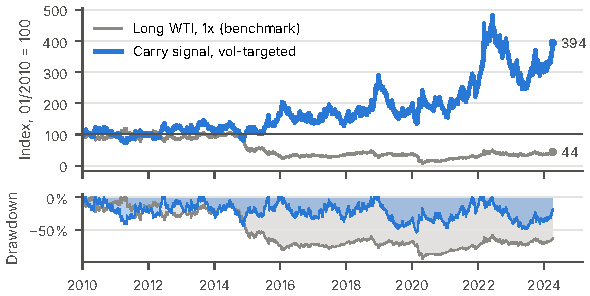
\includegraphics[width=\linewidth]{figures/fs_cumulative.pdf}

\head{Risk and performance, 01/2010--04/2024}
{\small\setlength{\tabcolsep}{6pt}\centering\begin{tabular}{@{}lrr@{}}
\toprule
Out-of-sample 01/2010--04/2024 & Strategy & Benchmark \\
\midrule
CAGR (total return) & 10.1\% & \textminus 5.6\% \\
Volatility p.a. & 35.6\% & 39.6\% \\
Sharpe ratio & 0.42 & 0.03 \\
Maximum drawdown & \textminus 54.0\% & \textminus 94.5\% \\
Calmar ratio & 0.19 & neg. \\
Skewness / excess kurtosis (daily) & 0.38 / 4.3 & \textminus 1.57 / 37.1 \\
Weekly hit rate & 49.6\% & 52.5\% \\
Avg. weekly win / loss & 4.0\% / \textminus 3.3\% & 3.3\% / \textminus 3.7\% \\
Beta / alpha p.a. vs benchmark & \textminus 0.24 / 15.3\% & 1.00 / -- \\
1-day VaR / ES 99\% (historical) & 5.6\% / 7.2\% & 6.1\% / 10.3\% \\
Time long / net exposure & 42\% / \textminus 0.09 & 100\% / 1.00 \\
Turnover p.a. (incl. rolls) & 38$\times$ & 24$\times$ \\
Trading-cost drag p.a. & 0.70\% & 0.47\% \\
\bottomrule
\end{tabular}
\par}

{\scriptsize\color{muted} After trading costs. Sharpe, volatility, VaR, ES: daily excess returns over T-bills. CAGR, drawdown: total returns incl.\ T-bill interest. Beta, alpha: regression on benchmark excess returns. EGARCH-$t$ 99\% VaR breaches: \NVarHitMain{} (Kupiec $p$ \NVarKupMain).}

\head{Calendar-year total return (2024: January--April)}
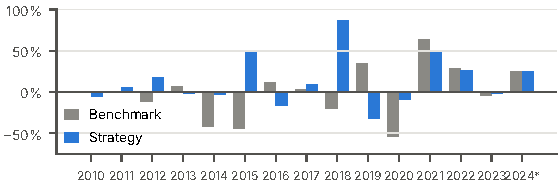
\includegraphics[width=\linewidth]{figures/fs_annual.pdf}

\head{Monthly total return of the strategy, \%}
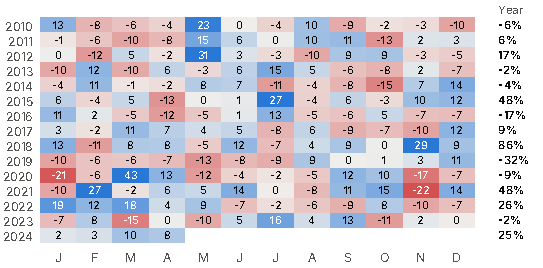
\includegraphics[width=\linewidth]{figures/fs_heatmap.pdf}
\end{minipage}

\vfill
\noindent{\color{rulegrey}\hrule}
\vspace{3pt}
{\scriptsize\color{muted}\textbf{Disclaimer.} Educational project for the Econometrics course of the MSc Innovative Finance, University of Liechtenstein. Not investment advice and not an offer of any financial product. Results are a historical simulation: they assume execution at daily settlement prices, the stated costs and no market impact, and they depend on modelling choices described in the report. Futures trading with leverage can lose more than the capital committed. Past and simulated performance are no guide to future results.}

\end{document}
